\section{Introduction}
\bjoern{What's the overall motivation for the project? What problem does it address?}
Increasingly, devices and services in our built environment are networked and can be controlled remotely. The proliferation of smart, controllable devices such as intelligent lighting, AV equipment, HVAC systems, or kitchen appliances raises the question of how to best interact with them. Prior work has introduced several approaches that use handheld mobile devices as {\em universal remote controls} to select and control appliances in the proximate environment- e.g., through pointing at such devices to select them, and through touch-screen or button interfaces to send control commands~\cite{beigl_point_1999,patel_2-way_2003}.

\bjoern{what are the drawbacks of this existing work?}
Some drawbacks of using handheld devices are that the device first has to be retrieved (e.g., from a pocket) and aimed; that two hands may be necessary for operation (one to hold the device, one to operate the touch screen); and that the user's visual attention is split between looking down at a screen and out at the device to-be-controlled. \bjoern{these all sound kind of weak.} \sean{When the number of smart devices increases, it also takes time to traverse within a list of dozens of items. In addition, mapping the name of a device to its real physical presence is not always intuitive. For example, it is hard to identify where is ``light in area E'' in an office building. Moreover, in a shared space, the person trying to control the device might not be the one that named it. } These general limitations have led researchers to investigate ``always-available'' physiological input modalities for phones on one hand~\cite{morris_emerging_2011}, and wearable computing devices on the other hand.

\begin{figure}[t]
\centering
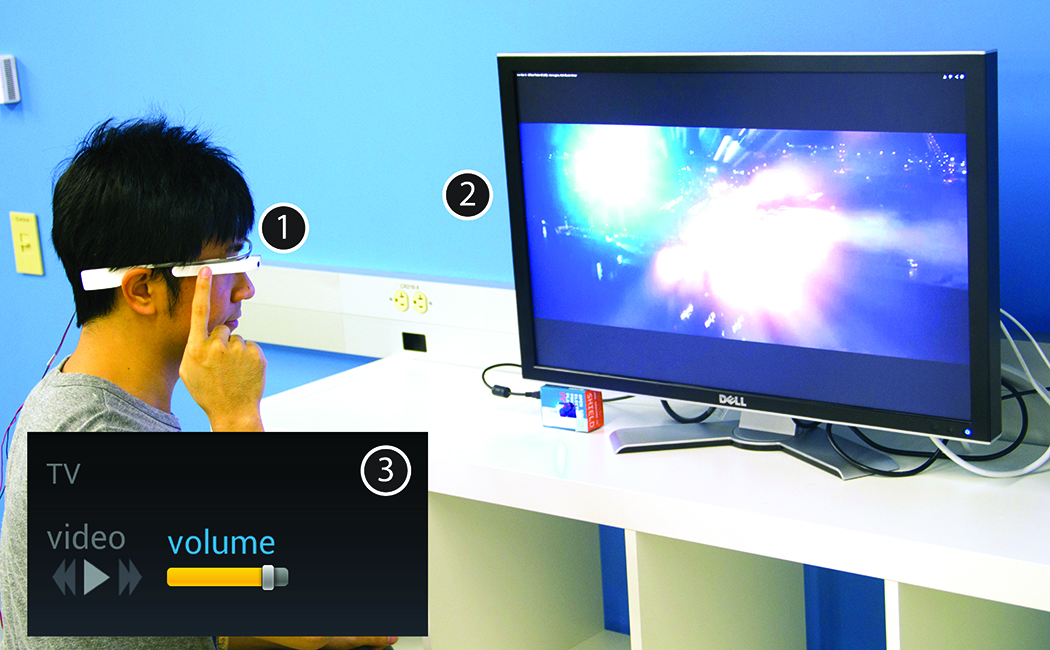
\includegraphics[width=1.0\columnwidth]{figures/teaser}
\caption{Teaser figure. Needs a caption.}
\label{fig:teaser}
\end{figure}

In this paper, we introduce a novel method for selecting and controlling smart appliances in physical spaces though the use of a head-worn computing device with near-eye display and wireless communication. We augment Google Glass\footnote{\url{http://www.google.com/glass/start/}} with custom hardware for this purpose. Users first look in the direction of the device they wish to control to initiate interaction (e.g., at a lamp to control lighting, or at a speaker to change music playback volume). If multiple devices fall within communication range, an on-screen disambiguation dialog lets users select a single target. Once acquired, a device specific control UI shown on the head-mounted display enables adjustment of discrete and continuous parameters through a touchpad interface (see Figure~\ref{fig:teaser}).

Our hardware relies on infrared communication between Glass and target devices to establish a connection; and on wireless ZigBee radio communication to exchange control messages.  Glass is augmented with a narrow IR emitter and a ZigBee ratio. Target devices similarly have IR receivers and ZigBee radios. These choices offer selection-through-head-orientation to initiate interaction; once initiated, users can look away from the target device while issuing control commands.

To understand the system performance, usability, and user experience of head-orientation targeting and head-mounted displays for device control, we first report measurements of the target range and accuracy of our device. We then conduct a comparative study of device acquisition time and error of different interface variants. We find that target acquisition through head orientation is faster than selecting items from a list, given the constraints of linear input using a head-worn touch controller. Finally, we report high-level feedback from $n$ users who use our system for home automation tasks.



